%%%%%%%%%%%%%%%%%%%%%%%%%%%%%%%%%%%%%%%%%
% Beamer Presentation
% LaTeX Template
% Version 1.0 (10/11/12)
%
% This template has been downloaded from:
% http://www.LaTeXTemplates.com
%
% License:
% CC BY-NC-SA 3.0 (http://creativecommons.org/licenses/by-nc-sa/3.0/)
%
%%%%%%%%%%%%%%%%%%%%%%%%%%%%%%%%%%%%%%%%%

%----------------------------------------------------------------------------------------
%	PACKAGES AND THEMES
%----------------------------------------------------------------------------------------

\documentclass[aspectratio=169,UTF8,11pt,t]{ctexbeamer}

\mode<presentation> {
\usetheme{Madrid}
\setbeamertemplate{footline}[frame number] % To remove the footer line in all slides
\setbeamercolor{page number in head/foot}{fg=blue}
\setbeamertemplate{navigation symbols}{} % To remove the navigation symbols from the bottom of all slides
}

% User Defined Block %%%%%%%%%%%%%%%%%%%%%%%%%%%%%%%%%%%%%%%%%%%%%%%%%%%%%%%%
\usepackage{setspace}
\definecolor{hanblue}{rgb}{0.27, 0.42, 0.81}
\definecolor{indiagreen}{rgb}{0.07, 0.53, 0.03}
\definecolor{indianred}{rgb}{0.8, 0.36, 0.36}
\definecolor{indianyellow}{rgb}{0.89, 0.66, 0.34}
\definecolor{babypink}{rgb}{0.96, 0.76, 0.76}
\definecolor{ao(english)}{rgb}{0.0, 0.5, 0.0}
\setbeamerfont{block title}{size=\normalsize}
\setbeamerfont{block body}{size=\small}
\newenvironment<>{blueblock}[1]{%
  \setbeamercolor{block title}{fg=white,bg=hanblue}%
  \begin{block}#2{#1}}{\vspace{-2mm}\end{block}}
\newenvironment<>{greenblock}[1]{%
  \setstretch{1.3}\setbeamercolor{block title}{fg=white,bg=indiagreen}%
  \begin{block}#2{#1}}{\end{block}}
\newenvironment<>{redblock}[1]{%
  \setstretch{1.3}\setbeamercolor{block title}{fg=white,bg=indianred}%
  \begin{block}#2{#1}}{\end{block}}
\newenvironment<>{yellowblock}[1]{%
  \setstretch{1.3}\setbeamercolor{block title}{fg=white,bg=indianyellow}%
  \begin{block}#2{#1}}{\end{block}}

%----------------------------------------------------------------------------------------
%	PACKAGES
%----------------------------------------------------------------------------------------
\usepackage{graphicx} % Allows including images
%\usepackage{tikz}
%\usetikzlibrary{shapes.geometric, arrows}
\usepackage{listings}
\lstset{language=C++,
    columns=flexible,
    basicstyle=\footnotesize\ttfamily,                                      % 设定代码字体、大小
    %numbers=left,xleftmargin=2em,framexleftmargin=2em,                   % 在左侧显示行号
    %numberstyle=\color{darkgray},                                        % 设定行号格式
    keywordstyle=\color{blue},                                            % 设定关键字格式
    commentstyle=\color{ao(english)},                                     % 设置代码注释的格式
    stringstyle=\color{brown},                                            % 设置字符串格式
    %showstringspaces=false,                                              % 控制是否显示空格
	%frame=lines,                                                         % 控制外框
    breaklines,                                                           % 控制是否折行
    postbreak=\space,                                                     % 控制折行后显示的标识字符
    breakindent=5pt,                                                      % 控制折行后缩进数量
    emph={size\_t,array,deque,list,map,queue,set,stack,vector,string,pair,tuple,constexpr}, % 非内置类型
    emphstyle={\color{teal}},
    escapeinside={(*@}{@*)},
}

\usepackage{tikz,tikz-layers}

%----------------------------------------------------------------------------------------
%	TITLE PAGE
%----------------------------------------------------------------------------------------

\title[\textit{C++程序设计:第七章}]{第七章~模板与泛型编程} % The short title appears at the bottom of every slide, the full title is only on the title page

%\author[李长河]{李长河} % Your name
%\institute[CUG] % Your institution as it will appear on the bottom of every slide, may be shorthand to save space
%{
%中国地质大学(武汉)\\ % Your institution for the title page
%\medskip
%\textit{lichanghe@cug.edu.cn} % Your email address
%}
\date{2020年10月26日} % Date, can be changed to a custom date

\begin{document}

%----------------------------------------------------------------------------------------
%	TIKZ FLOWCHART
%----------------------------------------------------------------------------------------
%\tikzstyle{startstop} = [rectangle, rounded corners, minimum width=2cm, minimum height=0.5cm, text centered, draw=black, fill=red!30, font=\tiny]
%\tikzstyle{io} = [trapezium, trapezium left angle=70, trapezium right angle=110, minimum width=0cm, minimum height=0cm, text centered, draw=black, fill=blue!30, font=\tiny]
%\tikzstyle{process} = [rectangle, minimum width=2.5cm, minimum height=1.5cm, text centered, draw=black, fill=orange!30, font=\tiny, text width=2cm]
%\tikzstyle{decision} = [diamond, minimum width=2.5cm, minimum height=2cm, text centered, draw=black, fill=green!30, font=\tiny, text width=1.8cm, aspect=1.1]


\begin{frame}
\titlepage % Print the title page as the first slide
\end{frame}


\begin{frame}[fragile]{代码复用}
\begin{tikzpicture}[remember picture,overlay]
% draw image
\node[inner sep=0] at (current page.center)
{
\includegraphics[scale=0.5]{影响开发效率因素.jpg}};
\visible<2->{\draw[red] (3.3,-2.3) rectangle (12,-1.6);}
\visible<3->{\draw[red,line width =2pt] (4.5,-2.0) -- (5.4,-2.0);}
\end{tikzpicture}
\end{frame}


\begin{frame}{目录}
\tableofcontents
\end{frame}

%----------------------------------------------------------------------------------------
%	PRESENTATION SLIDES
%----------------------------------------------------------------------------------------

%--------------------

\begin{frame}[fragile,c]{~} % Table of contents slide, comment this block out to remove it

\begin{block}{学习目标}
\begin{enumerate}
  \item 掌握模板的定义和基本使用方法,包括函数模板和类模板;
  \item 学会运用模板{\color{red}实现泛型编程};
  \item 掌握常用{\color{red}排序算法}和{\color{red}二分查找算法}。
\end{enumerate}
\end{block}

% ------功能模块说明,请注释掉-------
%\begin{columns}[t]
%\column{0.15\textwidth}
%\begin{block}{概念}
%\end{block}
%\column{0.15\textwidth}
%\begin{blueblock}{代码}
%\end{blueblock}
%\column{0.15\textwidth}
%\begin{yellowblock}{说明}
%\end{yellowblock}
%\column{0.15\textwidth}
%\begin{greenblock}{问题/答案}
%\end{greenblock}
%\column{0.15\textwidth}
%\begin{redblock}{注意}
%\end{redblock}
%\end{columns}
% ------功能模块说明,请注释掉-------

\end{frame}

%%--------------------

%#####################################
\section{函数模板}
%#####################################



%-------------------------------------

\begin{frame}[fragile]{7.1~函数模板}

\begin{block}{泛型编程}
\begin{itemize}
  \item 一种采用与数据类型无关的方式编写代码的方法,是\alert{代码重用}的重要手段。\onslide<2->{如何设计一个通用的排序算法?}
  \item <3->\alert{模板}是泛型编程的基础,它将数据类型参数化,为数据结构和算法的\alert{抽象}提供\alert{通用的代码}解决方案
\end{itemize}

\end{block}

\vspace{1mm}

\uncover<3->{请观察下面两组代码:}

\vspace{-4mm}

\begin{columns}[t]

\column{0.65\textwidth}
\begin{blueblock}<3->{\texttt{getMax}函数定义一}
\vspace{-1.5mm}\begin{lstlisting}
const int& getMax(const int &a, const int &b){
    return a>b ? a : b;
}
\end{lstlisting}\vspace{-1.5mm}
\end{blueblock}
\begin{blueblock}<3->{\texttt{getMax}函数定义二}
\vspace{-1.5mm}\begin{lstlisting}
const string& getMax(const string &a, const string &b){
    return a>b ? a : b;
}
\end{lstlisting}\vspace{-1.5mm}
\end{blueblock}

\column{0.3\textwidth}
\begin{greenblock}<4->{问题}
\begin{itemize}
  \item 两个函数定义有什么异同?
  \item <5-> 有什么办法可以简化?
\end{itemize}

\end{greenblock}

\end{columns}

\end{frame}

%-------------------------------------
\subsection{定义函数模板}
%-------------------------------------

\begin{frame}[fragile]{7.1.1~定义函数模板}

定义\alert{函数模板}来实现\alert{一类}函数的\alert{通用}代码解决方案,即实现某种功能的一类函数的抽象:

\vspace{-4mm}

\begin{columns}[t]

\column{0.65\textwidth}
\begin{blueblock}{\texttt{getMax}函数模板定义}

\begin{lstlisting}[moreemph={T}]
const int& getMax(const int &a, const int &b){
    return a>b ? a : b;
}
\end{lstlisting}
\begin{tikzpicture}[overlay]
\node at (5., 0.3) [rectangle, draw=blue!50, fill=blue!20, text=blue!70] {类型参数化};
\draw[->,blue,line width =1pt] (1.1,1.2) -- (2.8,-0.2);
\draw[->,blue,line width =1pt] (3.8,1.2) -- (2.9,-0.2);
\draw[->,blue,line width =1pt] (5.9,1.2) -- (3.0,-0.2);
\end{tikzpicture}
\begin{lstlisting}[moreemph={T}]
template <typename T>
const T& getMax(const T &a, const T &b){
    return a>b ? a : b;
}
\end{lstlisting}

\end{blueblock}

\begin{redblock}<3->{注意}
\begin{itemize}
  \item 注意不要混淆\alert{模板参数}和\alert{函数形参}的概念
  \item 模板的声明和定义应放在同一个头文件里
\end{itemize}
\end{redblock}

\column{0.3\textwidth}
\begin{yellowblock}<2->{说明}
$\bullet$ 模板的定义以关键字~\alert{\texttt{template}}~开始\\
$\bullet$ 模板参数列表放在一对\alert{尖括号}里面\\
$\bullet$ 每一个参数前面用\\\alert{\texttt{typename}}~或~\alert{\texttt{class}}~声明\\
$\bullet$ 列表含有多个模板参数则参数之间用\alert{逗号}分开
\end{yellowblock}

\end{columns}
\end{frame}

%-------------------------------------
\subsection{实例化函数模板}
%-------------------------------------

\begin{frame}[fragile]{7.1.2~实例化函数模板\small{~---~模板参数推断}}

如何使用函数模板? \onslide<2->{实例化模板函数,需要提供具体的\alert{数据类型或值}}

\vspace{-4mm}

\begin{columns}[t]

\column{0.65\textwidth}
\begin{blueblock}<3->{实例化方法一:隐式推断类型}
\begin{lstlisting}
cout << getMax(1.0, 2.5) << endl; // T被推断为double
\end{lstlisting}
生成如下函数实例
\begin{lstlisting}
const double& getMax(const double &a, const double &b){
    return a>b ? a : b;
}
\end{lstlisting}

\end{blueblock}
\begin{blueblock}<4->{实例化方法二:显式指定类型}
\begin{lstlisting}
cout << getMax<double>(1.0, 2.5) << endl;       //显式指明T为 double
cout << getMax<string>("Hi ", "C++") << endl;   //显式指明T为 string
\end{lstlisting}
\end{blueblock}

\column{0.3\textwidth}
\begin{yellowblock}<3->{说明}
编译器在\alert{编译}的过程中,利用实参来推断模板参数的类型
\end{yellowblock}
\vspace{1.8cm}
\begin{yellowblock}<4->{说明}
用户显式地指明模板参数的类型
\end{yellowblock}

\end{columns}

\end{frame}

%-----------------

\begin{frame}[fragile]{7.1.2~实例化函数模板\normalsize{~---~为类类型添加模板支持}}

当模板函数的实参为\alert{类类型}时,需要为类对象添加模板使用到的相关操作:

\vspace{-4mm}

\begin{columns}[t]
\column{0.65\textwidth}
\begin{blueblock}<2->{示例代码}
\begin{lstlisting}[moreemph={Fraction}]
Fraction a(3,4),b(2,5);
cout << getMax(a, b) << endl; // T为Fraction类型
\end{lstlisting}
\end{blueblock}

\begin{blueblock}<3->{函数模板实例化}
\begin{lstlisting}
const Fraction& getMax(const Fraction &a, const Fraction &b){
    return a>b ? a : b;
}
\end{lstlisting}
\end{blueblock}

\column{0.3\textwidth}
\begin{greenblock}<4->{问题}
在编译上面代码时提示编译错误,原因可能是什么?
\end{greenblock}
\begin{greenblock}<5->{答案}
在\texttt{getMax}模板内部用到了关系\texttt{>}运算,但\texttt{Fraction}类不支持关系\texttt{>}运算
\end{greenblock}
\end{columns}

\end{frame}

%-----------------

\begin{frame}[fragile]{7.1.2~实例化函数模板\normalsize{~---~为类类型添加模板支持}}

给\texttt{Fraction}类型添加关系\texttt{>}运算支持:

\vspace{-4mm}

\begin{columns}[t]
\column{0.65\textwidth}
\begin{blueblock}{\texttt{Fraction}类~关系\texttt{>}运算~声明及定义}
\begin{lstlisting}[moreemph={Fraction}]
class Fraction{
    // 将关系>运算声明为Fraction类的友元
    friend bool operator>(const Fraction &lhs, const Fraction &rhs);
    // 其它成员与之前一致
    ...
};

bool operator>(const Fraction &lhs, const Fraction &rhs){
    return lhs.m_numerator*rhs.m_denominator > lhs.m_denominator*rhs.m_numerator;
}
\end{lstlisting}
\end{blueblock}
\column{0.3\textwidth}
\begin{yellowblock}{说明}
根据运算符重载的原则将关系运算符函数\texttt{operator>}作为\texttt{Fraction}类的辅助函数,并将其声明为\texttt{Fraction}类的友元
\end{yellowblock}
\end{columns}

\end{frame}

%-------------------------------------
\subsection{模板参数类型}
%-------------------------------------

\begin{frame}[fragile]{7.1.3~模板参数类型}

以下两组代码中,函数\alert{模板参数}有什么异同?

\vspace{-4mm}

\begin{columns}[t]
\column{0.65\textwidth}
\begin{blueblock}{\texttt{foo}函数定义}
\begin{tikzpicture}[overlay]
  \visible<2->{\draw[red] (3.3,-0.6)--(4.8,-0.6);}
\end{tikzpicture}
\begin{lstlisting}[moreemph={T,U}]
template <typename T, typename U>
T foo(const T &t, const U &u) {
    return T(t);
}
\end{lstlisting}
\end{blueblock}
\begin{blueblock}{\texttt{maxElem}函数定义}
\begin{tikzpicture}[overlay]
  \visible<2->{\draw[red] (3.1,-0.6)--(4.5,-0.6);}
\end{tikzpicture}
\begin{lstlisting}[moreemph={T}]
template<typename T, int size>
const T& maxElem(T (&arr)[size]) {
    T *p = &arr[0];
    for (auto i = 0; i < size; ++i)
        if (*p < arr[i])
            p = &arr[i];
    return *p;
}
\end{lstlisting}
\end{blueblock}


\column{0.3\textwidth}
\begin{block}<2->{类型参数}
作为\alert{类型说明符},指定函数的返回值类型、形参类型以及函数体内对象的类型等
\end{block}
\begin{block}<2->{非类型参数}
代表一个值,当编译器实例化该模板时必须要为其提供一个\alert{常量}表达式
\end{block}
\begin{yellowblock}<3->{说明}
\texttt{maxElem}函数模板中的函数形参\texttt{arr}为一个指向含有\texttt{size}个\texttt{T}类型数据元素数组的引用
\end{yellowblock}
\end{columns}

\end{frame}

%-------------------

\begin{frame}[fragile]{7.1.3~模板参数类型}

调用\texttt{maxElem}函数:

\vspace{-4mm}

\begin{columns}[t]

\column{0.65\textwidth}
\begin{blueblock}{\texttt{maxElem}函数模板实例化}
\begin{lstlisting}
int arr[10] = {1,8,5,3};
int x = maxElem(arr);
// 或者显式调用 maxElem<int,10>(arr);
\end{lstlisting}
\end{blueblock}
编译器将会生成如下版本的函数:
\begin{blueblock}{}
\vspace{-2.5mm}\begin{lstlisting}
const int& maxElem(int (&arr)[10]);
\end{lstlisting}\vspace{-2mm}
\end{blueblock}

\column{0.3\textwidth}
\begin{greenblock}<2->{问题}
传递数组参数还有什么方式?
\end{greenblock}
\begin{greenblock}<3->{答案}
还可以通过指针传递数组首地址的方式
\end{greenblock}

\end{columns}

\end{frame}

%------------------

\begin{frame}[fragile]{7.1.3~模板参数类型\normalsize{~---~模板重载与特化}}

如果前面定义的\texttt{getMax}函数模板在调用过程中的实参为指针类型:

\vspace{-4mm}

\begin{columns}[t]

\column{0.65\textwidth}
\begin{blueblock}{\texttt{getMax}函数调用一}
\begin{lstlisting}[moreemph={T}]
int a = 1, b = 2;
getMax(&a, &b);
\end{lstlisting}
\end{blueblock}
\begin{blueblock}{\texttt{getMax}定义一}
\begin{lstlisting}[moreemph={T}]
template <typename T>
const T& getMax(const T &a, const T &b){
    return a > b ? a : b;
}
\end{lstlisting}
\begin{tikzpicture}[overlay]
  \visible<3->{\draw[blue,->,line width=1.5pt] (2,0.5)--(2,0);}
\end{tikzpicture}
\begin{onlyenv}<3->
\begin{lstlisting}[moreemph={T}]
const int* & getMax(const int* &a, const int* &b){
    return a > b ? a : b;
}
\end{lstlisting}
\end{onlyenv}
\end{blueblock}

\column{0.3\textwidth}
\begin{yellowblock}{说明}
需要返回两个指针所指向的对象的比较结果
\end{yellowblock}
\begin{greenblock}{问题}
\texttt{getMax}函数模板的定义还能否满足要求?
\end{greenblock}
\begin{greenblock}<2->{答案}
不能。编译器推演出的参数\texttt{T}为\texttt{int*},函数体里面的操作变成了两个指针对象的比较
\end{greenblock}

\end{columns}

\end{frame}

%-----------------

\begin{frame}[fragile]{7.1.3~模板参数类型\normalsize{~---~模板重载与特化}}

为此,需要\alert{重载}一个\texttt{getMax}模板函数:

\vspace{-4mm}

\begin{columns}[t]

\column{0.65\textwidth}
\begin{blueblock}{\texttt{getMax}函数调用二}
\begin{lstlisting}[moreemph={T}]
int a = 1, b = 2;
getMax(&a, &b);
\end{lstlisting}
\end{blueblock}
\begin{blueblock}{\texttt{getMax}函数模板重载}
\begin{lstlisting}[moreemph={T}]
template <typename T>
T* const & getMax( T* const &a, T* const &b){
    return *a>*b ? a : b;
}
\end{lstlisting}
\end{blueblock}

\column{0.3\textwidth}
\begin{yellowblock}{说明}
模板实参\texttt{T}的类型为\texttt{int},\texttt{*a}和\texttt{*b}指向的是\texttt{int}对象,函数体里面的操作是两个\texttt{int}对象的比较
\end{yellowblock}

\end{columns}

\end{frame}

%-----------------

\begin{frame}[fragile]{7.1.3~模板参数类型\normalsize{~---~模板重载与特化}}

进一步,如果调用的实参是指向字符串常量的指针:

\vspace{-4mm}

\begin{columns}[t]

\column{0.65\textwidth}
\begin{blueblock}{\texttt{getMax}函数调用三}
\begin{lstlisting}[moreemph={T}]
const char *a = "Hi", *b = "C++";
cout << getMax(a, b) << endl;
\end{lstlisting}
\end{blueblock}
\begin{blueblock}{\texttt{getMax}函数定义二}
\vspace{-2.5mm}\begin{lstlisting}[moreemph={T}]
template <typename T>
const T & getMax(const T &a, const T &b){
    return a > b ? a : b;
}

template <typename T>
T* const & getMax( T* const &a, T* const &b){
    return *a>*b ? a : b;
}
\end{lstlisting}\vspace{-2mm}
\end{blueblock}

\column{0.3\textwidth}
\begin{yellowblock}{说明}
需要返回指向字符串值较大的字符指针
\end{yellowblock}
\begin{greenblock}<2->{问题}
现有的两个\texttt{getMax}函数的定义还能否满足要求?
\end{greenblock}
\begin{greenblock}<3->{答案}
不能。\texttt{*a}和\texttt{*b}指向的是单个字符,函数体里面的操作变成了两个字符的比较
\end{greenblock}

\end{columns}

\end{frame}

%-----------------

\begin{frame}[fragile]{7.1.3~模板参数类型\normalsize{~---~模板重载与特化}}

为此,需要\alert{特例化}一个\texttt{getMax}模板函数:

\vspace{-4mm}

\begin{columns}[t]

\column{0.65\textwidth}
\begin{blueblock}{\texttt{getMax}函数调用三}
\begin{lstlisting}[moreemph={T}]
const char *a = "Hi", *b = "C++";
cout << getMax(a, b) << endl;
\end{lstlisting}
\end{blueblock}
\begin{blueblock}{\texttt{getMax}函数模板特化}
\begin{lstlisting}[moreemph={T}]
template <>
const char* const & getMax(const char* const &a, const char* const &b){
    return strcmp(a,b) > 0 ? a : b;
}
\end{lstlisting}
\end{blueblock}


\column{0.3\textwidth}
\begin{yellowblock}{说明}
模板参数列表为空,表明将显式提供所有模板实参
\end{yellowblock}
\vspace{-2mm}
\begin{yellowblock}{说明}
\texttt{T}被推断为\texttt{const char*},\texttt{a}和\texttt{b}分别为一个指向\texttt{const char}对象的\texttt{const}指针的引用,函数是对两个字符串值的比较
\end{yellowblock}
\vspace{-2mm}
\begin{greenblock}<2->{问题}
为什么会选择特例化的版本?
\end{greenblock}

\end{columns}

\end{frame}

%-----------------

\begin{frame}[fragile]{7.1.3~模板参数类型\normalsize{~---~模板重载与特化}}

还可以通过模板特化改善算法:

\vspace{-4mm}

\begin{columns}[t]

\column{0.65\textwidth}
\begin{blueblock}<2->{\texttt{Swap}函数模板定义}
\vspace{-2.5mm}\begin{lstlisting}[moreemph={T}]
template<typename T>
void Swap(T &a, T &b) {
    T c(a); // 复制构造对象 c
    a = b;
    b = c;
}
\end{lstlisting}\vspace{-2mm}
\end{blueblock}

\column{0.3\textwidth}
\begin{yellowblock}<2->{说明}
需要构造一个辅助的局部对象\texttt{c},才能完成\texttt{a}和\texttt{b}的交换
\end{yellowblock}

\end{columns}

\vspace{4mm}

\uncover<3->{如果\texttt{T}是\texttt{int},可以利用模板特化做出优化:}

\vspace{-4mm}

\begin{columns}[t]

\column{0.65\textwidth}
\begin{blueblock}<4->{\texttt{Swap}函数模板特化}
\vspace{-2.5mm}\begin{lstlisting}[moreemph={T}]
template<>
void Swap(int &a, int &b)
    a ^= b;
    b ^= a;
    a ^= b;
}
\end{lstlisting}\vspace{-2mm}
\end{blueblock}

\column{0.3\textwidth}
\begin{yellowblock}<4->{说明}
利用异或操作完成两个整数的交换,没有创建辅助对象,没有产生构造和析构行为,提高了执行效率
\end{yellowblock}

\end{columns}

\end{frame}

%-----------------

%-------------------------------------
\subsection{类成员模板}
%-------------------------------------

%-----------------
\begin{frame}[fragile]{7.1.4~类成员模板}

类的成员函数也可以定义为函数模板:

\vspace{-4mm}

\begin{columns}[t]

\column{0.65\textwidth}
\begin{blueblock}{类\texttt{X}定义}
\begin{lstlisting}[moreemph={T}]
class X{
    void * m_p = nullptr;
public:
    template <typename T>
    void reset(T *t) { m_p = t; }
};
\end{lstlisting}
\end{blueblock}
\begin{blueblock}<2->{\texttt{reset}函数调用}
\begin{lstlisting}[moreemph={T}]
int i = 0;
double d = 0;
X x;
x.reset(&i); // 或者x.reset<int>(&i);
x.reset(&d); // 或者x.reset<double>(&d);
\end{lstlisting}
\end{blueblock}

\column{0.3\textwidth}
\begin{yellowblock}{说明}
成员函数\texttt{reset}定义为一个函数模板,接受不同类型的指针实参
\end{yellowblock}
\begin{yellowblock}<2->{说明}
$\bullet$ 第一条\texttt{reset}函数调用中\texttt{T}被推断为\texttt{int}类型,\texttt{m\_p}存放整型对象\texttt{i}的地址\\
$\bullet$ 第二条\texttt{reset}函数调用中\texttt{T}被推断为\texttt{double}类型,\texttt{m\_p}存放\texttt{double}类对象\texttt{d}的地址
\end{yellowblock}

\end{columns}

\end{frame}
%-----------------



%-------------------------------------
\subsection{可变参函数模板}
%-------------------------------------

\begin{frame}[fragile]{7.1.5~可变参函数模板}

C++11新标准允许我们使用\alert{数目可变}的模板参数:

\vspace{-4mm}

\begin{columns}[t]

\column{0.65\textwidth}
\begin{blueblock}{\texttt{foo}函数定义}
\begin{lstlisting}[moreemph={T}]
template<typename... Args >
    void foo(Args... args) {
    // 打印参数包args中参数的个数
    cout << sizeof...(args) << endl;
}
\end{lstlisting}
\end{blueblock}
\begin{blueblock}<2->{\texttt{foo}函数调用}
\begin{lstlisting}[moreemph={T}]
foo(); // 输出:0
foo(1,1.5); // 输出:2
foo(1,1.5,"C++"); // 输出:3
\end{lstlisting}
\end{blueblock}

\column{0.3\textwidth}
\begin{yellowblock}{说明}
$\bullet$ 可变数目的参数称为\alert{参数包},用省略号“\alert{\texttt{...}}”表示,可包含0到任意个模板参数\\
$\bullet$ \texttt{foo}函数的形参\texttt{args}为模板参数包类型,接受可变数目的实参
\end{yellowblock}

\end{columns}

\end{frame}

\begin{frame}[fragile]{7.1.5~可变参函数模板\normalsize{~---~转发参数包}}
\begin{block}{在泛型编程中,常常需要将参数原封不动的转发给另外一个函数}
\begin{tikzpicture}[overlay]
\visible<2->{\draw[color=red!70,->,line width=1.5pt] (6.5,-2) -- node [color=red!70,pos=0.45,above,sloped]{改进效率}(8,-2);} 
\end{tikzpicture}
\begin{columns}
\column{0.4\textwidth}
\begin{lstlisting}[moreemph={T}]
template<typename TYPE, typename ARG>
TYPE* get_instance(const ARG arg){

     TYPE *ret;
     ret = new TYPE(arg);
     return ret;
}
\end{lstlisting}
\column{0.4\textwidth}
\begin{onlyenv}<2->
\begin{lstlisting}[moreemph={T}]
template<typename TYPE, typename ARG>
TYPE* get_instance(const ARG &arg){

     TYPE *ret;
     ret = new TYPE(arg);
     return ret;
}
\end{lstlisting}
\end{onlyenv}
\end{columns}
\end{block}

\begin{greenblock}<3->{问题}
如果参数类型是右值,如何处理?
\end{greenblock}
\end{frame}
\begin{frame}[fragile]{7.1.5~可变参函数模板\normalsize{~---~转发参数包}}

两个函数的形参都是\alert{右值引用},\texttt{forwardValue}函数调用报错,为什么?

\vspace{-4mm}

\begin{columns}[t]

\column{0.65\textwidth}
\begin{blueblock}{\texttt{forwardValue}函数及\texttt{rvalue}函数定义}
\vspace{-2mm}\begin{lstlisting}[moreemph={T}]
void rvalue(int &&val){}

template<typename T>
void forwardValue(T &&val) {
    rvalue(val);
}
\end{lstlisting}\vspace{-2mm}
\end{blueblock}
\begin{blueblock}{\texttt{forwardValue}函数调用}
\vspace{-2mm}\begin{lstlisting}[moreemph={T}]
forwardValue(42);   // 错误
\end{lstlisting}\vspace{-2mm}
\end{blueblock}
\begin{blueblock}<2->{\texttt{forwardValue}函数调用细节}
\vspace{-2mm}\begin{lstlisting}[moreemph={T}]
T &&val = 42;       //等同于auto &&val = 42
rvalue(val);
\end{lstlisting}\vspace{-2mm}
\end{blueblock}

\column{0.3\textwidth}
\begin{greenblock}<2->{答案}
$\bullet$ 右值引用声明 \texttt{\&\&}与类型推导结合可以与右值绑定,所以\texttt{val}为右值引用\\
$\bullet$ 右值引用\texttt{val}引用右值42,但\alert{\texttt{val}本身是左值}\\
$\bullet$ \texttt{rvalue}函数只接受右值形参,但\texttt{val}是左值
\end{greenblock}
\begin{greenblock}<3->{问题}
可以让传入\texttt{rvalue}函数的\alert{实参保持原属性吗}?
\end{greenblock}

\end{columns}

\end{frame}
%-----------------

\begin{frame}[fragile]{7.1.5~可变参函数模板\normalsize{~---~转发参数包}}

在C++11新标准下可以利用~\alert{\texttt{std::forward}}~函数实现:

\vspace{-4mm}

\begin{columns}[t]

\column{0.65\textwidth}
\begin{blueblock}{\texttt{std::forward}转发左值描述性声明}
\vspace{-2mm}\begin{lstlisting}[basicstyle=\scriptsize\ttfamily,moreemph={T}]
template<typename T>
T&& forward( typename std::remove_reference<T>::type& t );
\end{lstlisting}\vspace{-2mm}
\end{blueblock}
\begin{blueblock}<2->{\texttt{forwardValue}函数定义二}
\vspace{-2mm}\begin{lstlisting}[moreemph={T}]
template<typename T>
void forwardValue(T &&val) {
    rvalue(std::forward<T>(val));
}
\end{lstlisting}\vspace{-2mm}
\end{blueblock}
\begin{blueblock}<2->{\texttt{forwardValue}函数调用二}
\vspace{-2mm}\begin{lstlisting}[moreemph={T}]
forwardValue(42);       //正确
int a = 42;
forwardValue(a);        //正确
\end{lstlisting}\vspace{-2mm}
\end{blueblock}

\column{0.3\textwidth}
\begin{yellowblock}<3->{说明}
$\bullet$ 当传入\texttt{forwardValue}的实参为右值,\texttt{T}被推断为非引用类型,forward<T>返回右值引用\\
$\bullet$ 当传入\texttt{forwardValue}的实参为左值,\texttt{T}被推断为左值引用类型,此时\texttt{forward<T>}将返回左值引用
\end{yellowblock}
\vspace{-2mm}
\begin{redblock}<4->{注意}
在C++11新标准下,\\
\texttt{\&\& \&和\& \&\&}折叠为 \texttt{\&}
\end{redblock}

\end{columns}

\end{frame}


 
%%###############################################################################
%\section{类模板}
%%###############################################################################
%
%%-----------------
%
%\begin{frame}[fragile]{7.2~类模板}
%
%类似函数模板,可以定义一个类模板用来生成具有\alert{相同结构}的一族类实例:
%
%\vspace{-4mm}
%
%\begin{columns}[t]
%
%\column{0.65\textwidth}
%\begin{blueblock}{\texttt{Array}类模板定义}
%\begin{lstlisting}[moreemph={T}]
%template<typename T, size_t N>
%class Array {
%    T m_ele[N];
%public:
%    Array() {}
%    Array(const std::initializer_list<T> &);
%    T& operator[](size_t i);
%    constexpr size_t size() { return N; }
%};
%\end{lstlisting}
%\end{blueblock}
%
%\column{0.3\textwidth}
%\begin{yellowblock}{说明}
%$\bullet$ 类型参数\texttt{T}和非类型参数\texttt{N},分别用来表示元素的类型和元素的数目\\
%$\bullet$ \alert{\texttt{initializer\_list}}~类型是C++11标准库提供的新类型,支持具有相同类型但数量未知的列表类型
%\end{yellowblock}
%
%\end{columns}
%
%\end{frame}
%
%%-----------------
%
%%-------------------------------------
%\subsection{成员函数定义}
%%-------------------------------------
%
%%-----------------
%
%\begin{frame}[fragile]{7.2.1~成员函数定义}
%
%与普通类相同,既可以在类的内部,也可以在\alert{类的外部}定义\alert{类模板成员函数}:
%
%\vspace{-4mm}
%
%\begin{columns}[t]
%
%\column{0.65\textwidth}
%\begin{blueblock}{\texttt{Array}类模板~构造函数~类外定义}
%\begin{lstlisting}[moreemph={T,Array,initializer}]
%template<typename T, size_t N>
%Array<T, N>::Array(const std::initializer_list<T> &l):m_ele{T()}{
%    size_t m = l.size() < N ? l.size() : N;
%    for (size_t i = 0; i < m; ++i) {
%        m_ele[i] = *(l.begin() + i);
%    }
%}
%\end{lstlisting}
%\end{blueblock}
%
%\column{0.3\textwidth}
%\begin{yellowblock}{说明}
%$\bullet$ 必须以关键字\texttt{template}开始,后接\alert{与类模板相同}的模板参数列表\\
%$\bullet$ 紧随类名后面的参数列表代表一个实例化的实参列表,每个参数不需要\texttt{typename}或\texttt{class}说明符
%\end{yellowblock}
%
%\end{columns}
%
%\end{frame}
%
%%-----------------
%
%\begin{frame}[fragile]{7.2.1~成员函数定义}
%
%与普通类相同,既可以在类的内部,也可以在\alert{类的外部}定义\alert{类模板成员函数}:
%
%\vspace{-4mm}
%
%\begin{columns}[t]
%
%\column{0.65\textwidth}
%\begin{blueblock}{\texttt{Array}类模板~构造函数~类外定义}
%\begin{lstlisting}[moreemph={T,Array,initializer}]
%template<typename T, size_t N>
%Array<T, N>::Array(const std::initializer_list<T> &l):m_ele{T()}{
%    size_t m = l.size() < N ? l.size() : N;
%    for (size_t i = 0; i < m; ++i) {
%        m_ele[i] = *(l.begin() + i);
%    }
%}
%\end{lstlisting}
%\end{blueblock}
%\begin{blueblock}<2->{\texttt{Array}类模板~\texttt{[]}运算符函数~类外定义}
%\begin{lstlisting}[moreemph={T,Array}]
%template<typename T, size_t N>
%T& Array<T, N>::operator[](size_t i) {
%    return m_ele[i];
%}
%\end{lstlisting}
%\end{blueblock}
%
%\column{0.3\textwidth}
%\begin{yellowblock}{说明}
%$\bullet$ \texttt{m\_ele}中的每一个元素用T类型的默认初始化方式(\texttt{T()})初始化\\
%$\bullet$ 将形参\texttt{l}中的元素依次复制到类模板数组成员\texttt{m\_ele}中相应的位置\\
%$\bullet$ \texttt{l.begin}返回列表\texttt{l}中第一个元素的迭代器
%\end{yellowblock}
%\begin{yellowblock}<2->{说明}
%类模板的下标运算符函数返回数组\texttt{m\_ele}中第\texttt{i}个元素的引用
%\end{yellowblock}
%
%\end{columns}
%
%\end{frame}
%
%%-----------------
%
%%-------------------------------------
%\subsection{实例化类模板}
%%-------------------------------------
%
%%-----------------
%
%\begin{frame}[fragile]{7.2.2~实例化类模板}
%
%当使用一个类模板时,我们需要\alert{显式}提供模板参数信息,即\alert{模板实参列表}:
%
%\vspace{-4mm}
%
%\begin{columns}[t]
%
%\column{0.65\textwidth}
%\begin{blueblock}{实例化\texttt{Array}类模板}
%\begin{lstlisting}[moreemph={Array}]
%Array<char, 5> a; //创建一个Array<char, 5>类型对象 a
%Array<int, 5> b = {1,2,3}; //创建一个Array<int, 5>类型对象 b
%\end{lstlisting}
%\end{blueblock}
%\uncover<2->{下面代码逐个输出对象\texttt{b}的每一个元素:}
%\begin{blueblock}<2->{}
%\begin{lstlisting}[moreemph={Array}]
%for (int i = 0; i < b.size(); ++i)
%    cout << b[i] << " ";
%\end{lstlisting}
%\end{blueblock}
%\uncover<2->{输出结果为:\texttt{1 2 3 0 0}}
%
%\column{0.3\textwidth}
%\begin{yellowblock}{说明}
%创建对象\texttt{b}时,将执行具有形参的构造函数,其形参\texttt{l}接受初始化列表 \texttt{\{1,2,3\}},其余元素具有默认值\texttt{0}
%\end{yellowblock}
%
%
%\end{columns}
%
%\end{frame}
%
%%-----------------
%
%%-------------------------------------
%\subsection{默认模板参数}
%%-------------------------------------
%
%%-----------------
%
%\begin{frame}[fragile]{7.2.3~默认模板参数}
%
%\alert{函数参数}可以具有默认值,\alert{模板参数}同样也可以有默认值:
%
%\vspace{-4mm}
%
%\begin{columns}[t]
%
%\column{0.65\textwidth}
%\begin{blueblock}{\texttt{Array}类模板定义二}
%\vspace{-1mm}\begin{lstlisting}[moreemph={Array,T,Less,F}]
%template<typename T = int, size_t N = 10>
%class Array {
%    // 其它成员保持不变
%};
%\end{lstlisting}\vspace{-1mm}
%\end{blueblock}
%\begin{blueblock}<2->{实例化\texttt{Array}类模板二}
%\begin{lstlisting}[moreemph={Array}]
%Array<> a = { 'A' };
%cout << a.size() << " " << a[0] << endl;
%\end{lstlisting}
%\end{blueblock}
%\uncover<2->{输出结果为:\texttt{10 65}}
%
%\column{0.3\textwidth}
%\begin{yellowblock}{说明}
%$\bullet$ \alert{类模板参数}~\texttt{T}具有默认类型\texttt{int}\\
%$\bullet$ \alert{类模板参数}~\texttt{N}具有默认值\texttt{10}
%\end{yellowblock}
%\begin{yellowblock}<2->{说明}
%$\bullet$ \texttt{a}的元素数目为默认值\texttt{10}\\
%$\bullet$ \texttt{a[0]}的类型为\texttt{int},字符\texttt{'A'}转换为\texttt{65}
%\end{yellowblock}
%
%\end{columns}
%
%\end{frame}
%
%%-----------------
%
%\begin{frame}[fragile]{7.2.3~默认模板参数}
%
%和\alert{类模板参数}一样,\alert{函数模板参数}也可以有默认值:
%
%\vspace{-4mm}
%
%\begin{columns}[t]
%
%\column{0.65\textwidth}
%\begin{blueblock}{\texttt{Array}类模板定义三}
%\vspace{-1mm}\begin{lstlisting}[moreemph={Array,T,Less,F}]
%template<typename T, size_t N>
%class Array {
%    // 其它成员保持不变
%public:
%    template<typename F = Less<T>>
%    void sort(F f = F());
%};
%\end{lstlisting}\vspace{-1mm}
%\end{blueblock}
%\begin{blueblock}<2->{\texttt{Less}类模板定义}
%\vspace{-1mm}\begin{lstlisting}[moreemph={Less,T}]
%template<typename T>
%struct Less{
%    bool operator()(const T &a, const T &b) {
%        return a < b;
%    }
%};
%\end{lstlisting}\vspace{-1mm}
%\end{blueblock}
%
%\column{0.3\textwidth}
%\begin{yellowblock}{说明}
%$\bullet$ 新增了一个成员函数模板\texttt{sort},用来对数组进行排序\\
%$\bullet$ \texttt{sort}的\alert{函数模板参数}~\texttt{F}具有默认值\texttt{Less<T>}
%\end{yellowblock}
%\begin{yellowblock}<2->{说明}
%类模板\texttt{Less<T>}具有一个模板参数\texttt{T},且只有一个函数调用运算符,该成员函数带有两个形参,用来比较两个形参的大小,返回值类型为\texttt{bool}
%\end{yellowblock}
%
%\end{columns}
%
%\end{frame}
%
%%-----------------
%
%\begin{frame}[fragile]{7.2.3~默认模板参数}
%
%和\alert{类模板参数}一样,\alert{函数模板参数}也可以有默认值:
%
%\vspace{-4mm}
%
%\begin{columns}[t]
%
%\column{0.65\textwidth}
%\begin{blueblock}{\texttt{Array}类模板定义三}
%\vspace{-1mm}\begin{lstlisting}[moreemph={Array,T,Less,F}]
%template<typename T, size_t N = 10>
%class Array {
%    // 其它成员保持不变
%public:
%    template<typename F = Less<T>>
%    void sort(F f = F());
%};
%\end{lstlisting}\vspace{-1mm}
%\end{blueblock}
%
%\column{0.3\textwidth}
%\begin{yellowblock}{说明}
%$\bullet$ \texttt{sort}的\alert{函数参数}~\texttt{f}也有默认值,即\texttt{F}类的一个函数对象,代表默认比较方式为\texttt{Less}
%\end{yellowblock}
%\begin{greenblock}<2->{问题}
%理清~\alert{函数参数}和\alert{模板参数}的概念
%\end{greenblock}
%
%\end{columns}
%
%\end{frame}
%
%%-----------------
%
%%###############################################################################
%\section{排序与查找}
%%###############################################################################
%
%%-------------------------------------
%\subsection{排序算法}
%%-------------------------------------
%
%%-----------------
%
%\begin{frame}[fragile]{7.3.1~排序算法}
%
%排序是数据处理的最基本任务,目的是按照某种规则将一组无序数据重新排列,使之有序。下面将给\texttt{Array}模板类增加三种最常用的排序算法:选择排序、插入排序和冒泡排序
%
%\vspace{-4mm}
%
%\begin{columns}[t]
%
%\column{0.65\textwidth}
%\begin{blueblock}<2->{\texttt{Array}类模板定义四}
%\vspace{-3mm}
%\begin{lstlisting}[moreemph={Array,T}]
%template<typename T, size_t N>
%class Array {
%    //其它成员保持不变
%public:
%    template<typename F = Less<T> >
%    void selectionSort(F f = F()); //选择排序
%    template<typename F = Less<T> >
%    void insertionSort(F f = F()); //插入排序
%    template<typename F = Less<T> >
%    void bubbleSort(F f = F()); //冒泡排序
%private:
%    void swap(int i, int j){
%        T t = m_ele[i];
%        m_ele[i] = m_ele[j];
%        m_ele[j] = t;
%    }
%};
%\end{lstlisting}
%\vspace{-3mm}
%\end{blueblock}
%
%\column{0.3\textwidth}
%\begin{yellowblock}<2->{说明}
%成员\texttt{swap}函数用来交换两个元素的位置,它仅在\texttt{Array}类内部使用,因此它的访问属性为\texttt{private}
%\end{yellowblock}
%
%\end{columns}
%
%\end{frame}
%
%%-----------------
%
%\begin{frame}[fragile]{7.3.1 排序算法\normalsize{~---~选择排序}}
%
%每次在待排序元素中选择最小的一个,换放到已排序数列后面
%
%\vspace{1mm}
%
%\begin{center}
%
\includegraphics[width=0.8\textwidth]{selection_sort_1}\\\vspace{3mm}
%\uncover<2->{
\includegraphics[width=0.8\textwidth]{selection_sort_2}}\\\vspace{-11mm}
%\uncover<3->{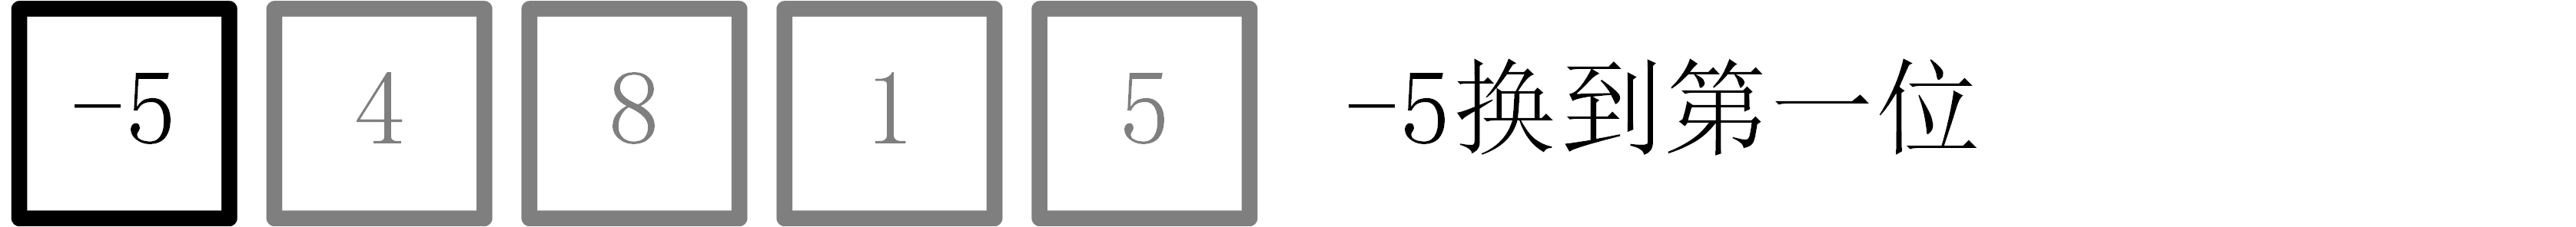
\includegraphics[width=0.8\textwidth]{selection_sort_3}}\\
%\uncover<4->{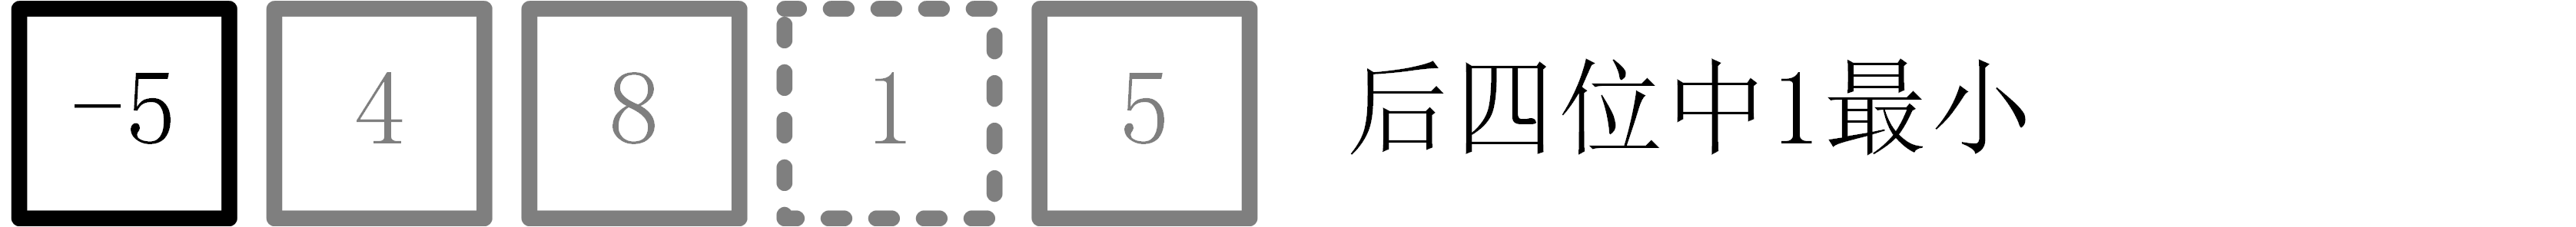
\includegraphics[width=0.8\textwidth]{selection_sort_4}}\\\vspace{-11mm}
%\uncover<5->{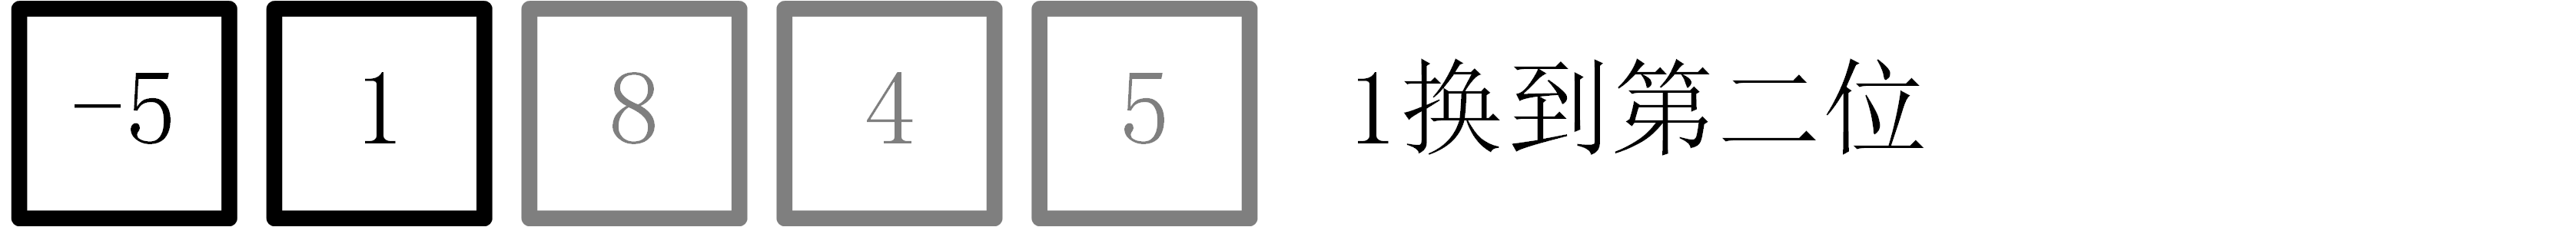
\includegraphics[width=0.8\textwidth]{selection_sort_5}}\\
%\uncover<6->{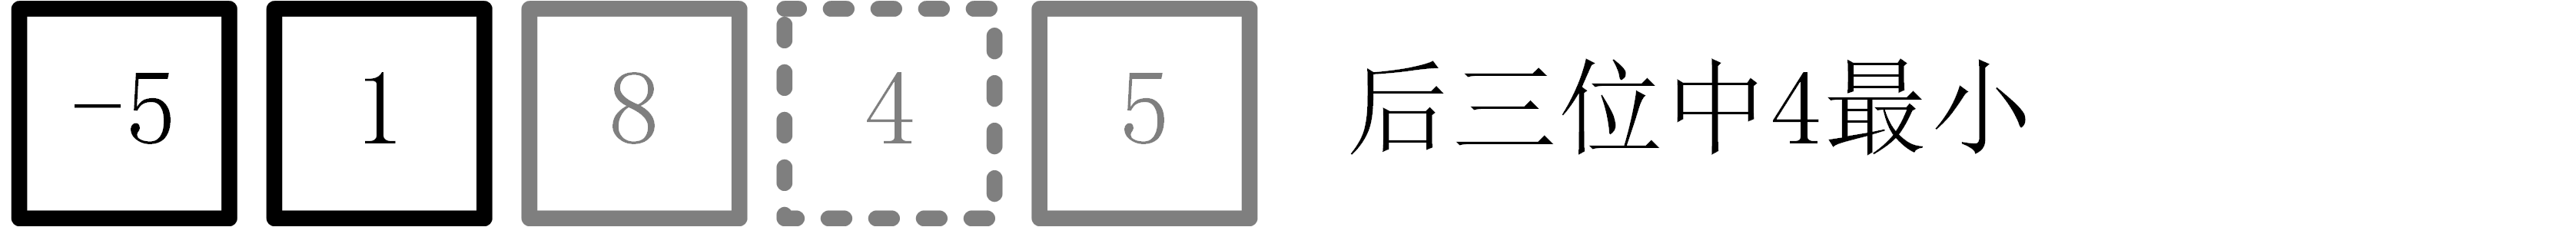
\includegraphics[width=0.8\textwidth]{selection_sort_6}}\\\vspace{-11mm}
%\uncover<7->{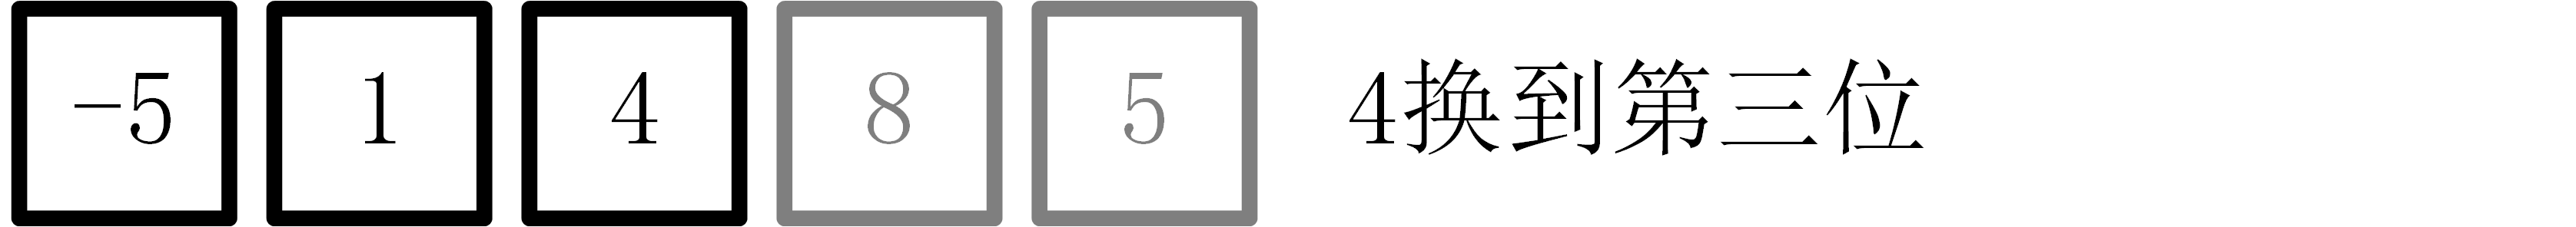
\includegraphics[width=0.8\textwidth]{selection_sort_7}}\\
%\uncover<8->{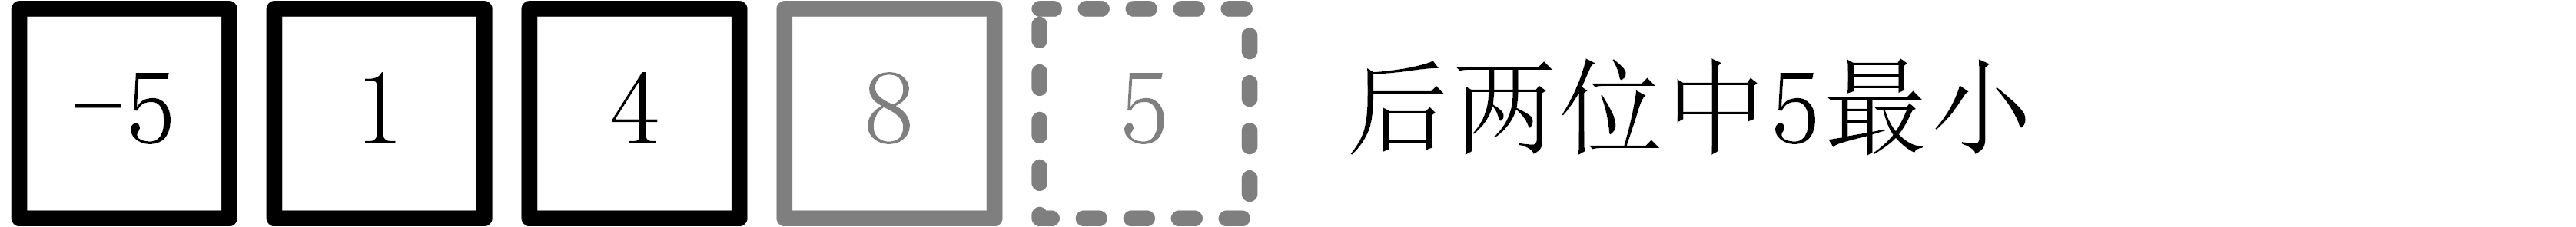
\includegraphics[width=0.8\textwidth]{selection_sort_8}}\\\vspace{-11mm}
%\uncover<9->{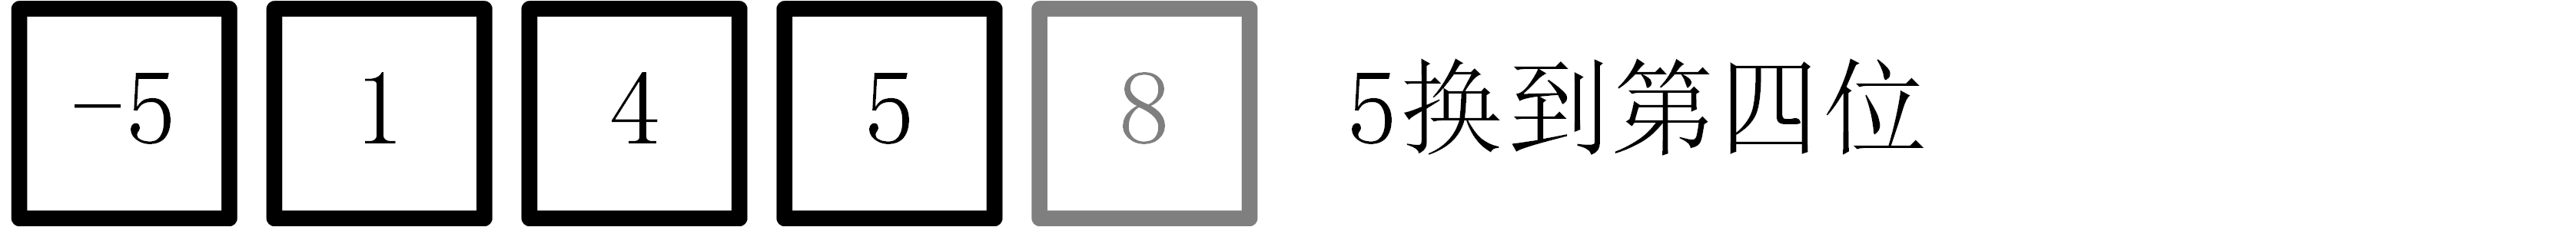
\includegraphics[width=0.8\textwidth]{selection_sort_9}}\\\vspace{3mm}
%\uncover<10->{
\includegraphics[width=0.8\textwidth]{selection_sort_10}}
%\end{center}
%
%\end{frame}
%
%%-----------------
%
%\begin{frame}[fragile]{7.3.1 排序算法\normalsize{~---~选择排序}}
%
%选择排序算法的实现如下:
%
%\vspace{-4mm}
%
%\begin{columns}[t]
%
%\column{0.65\textwidth}
%\begin{blueblock}{\texttt{Array}成员函数\texttt{selectionSort}定义}
%\begin{lstlisting}[moreemph={Array,T,F}]
%template<typename T, size_t N>
%template<typename F >
%void Array<T, N>::selectionSort(F f) {
%    for (int i = 0; i < N - 1; ++i){
%        int min = i; // 记录待排序数据中最小元素位置
%        for (int j = i + 1; j < N; ++j) {
%            if (f(m_ele[j], m_ele[min]))
%                min = j; //更新最小元素位置
%        }
%        swap(i, min); //把最小元素放到位置i
%    }
%}
%\end{lstlisting}
%\end{blueblock}
%
%\column{0.3\textwidth}
%\begin{yellowblock}{说明}
%\texttt{if}语句里的条件表达式将调用函数对象\texttt{f}(\texttt{Less<T>}),检查第一个实参对象是否小于第二个实参对象
%\end{yellowblock}
%
%\end{columns}
%
%\end{frame}
%
%%-----------------
%
%\begin{frame}[fragile]{7.3.1 排序算法\normalsize{~---~插入排序}}
%
%将待排序的元素逐个插入已经排好序的元素序列中
%
%\vspace{1mm}
%
%\begin{center}
%
\includegraphics[width=0.8\textwidth]{insertion_sort_1}\\\vspace{3mm}
%\uncover<2->{
\includegraphics[width=0.8\textwidth]{insertion_sort_2}}\\
%\uncover<3->{
\includegraphics[width=0.8\textwidth]{insertion_sort_3}}\\\vspace{-10.9mm}
%\uncover<4->{
\includegraphics[width=0.8\textwidth]{insertion_sort_4}}\\\vspace{-10.9mm}
%\uncover<5->{
\includegraphics[width=0.8\textwidth]{insertion_sort_5}}\\
%\uncover<6->{
\includegraphics[width=0.8\textwidth]{insertion_sort_6}}\\\vspace{-10.9mm}
%\uncover<7->{
\includegraphics[width=0.8\textwidth]{insertion_sort_7}}\\\vspace{-10.9mm}
%\uncover<8->{
\includegraphics[width=0.8\textwidth]{insertion_sort_8}}\\
%\uncover<9->{
\includegraphics[width=0.8\textwidth]{insertion_sort_9}}\\\vspace{-10.9mm}
%\uncover<10->{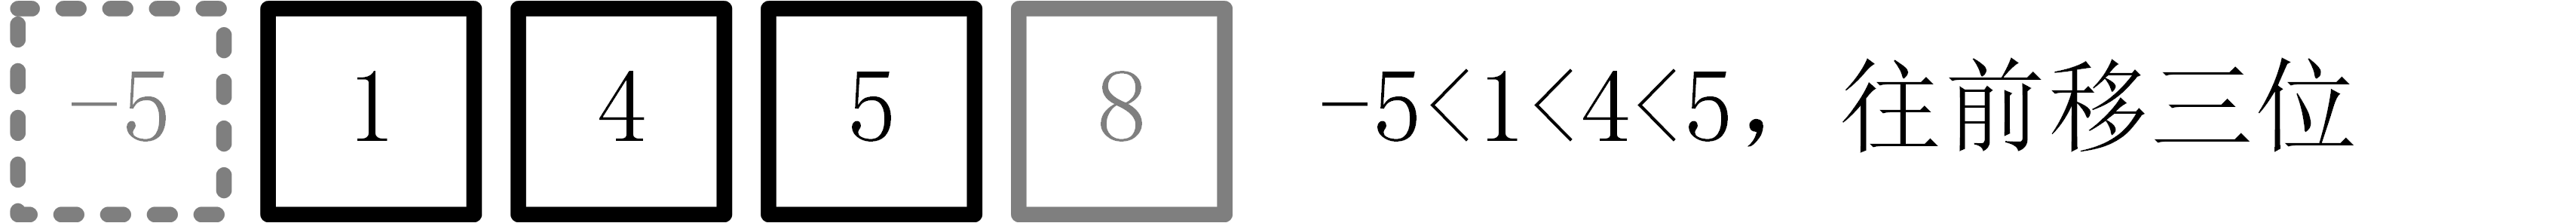
\includegraphics[width=0.8\textwidth]{insertion_sort_10}}\\\vspace{-10.9mm}
%\uncover<11->{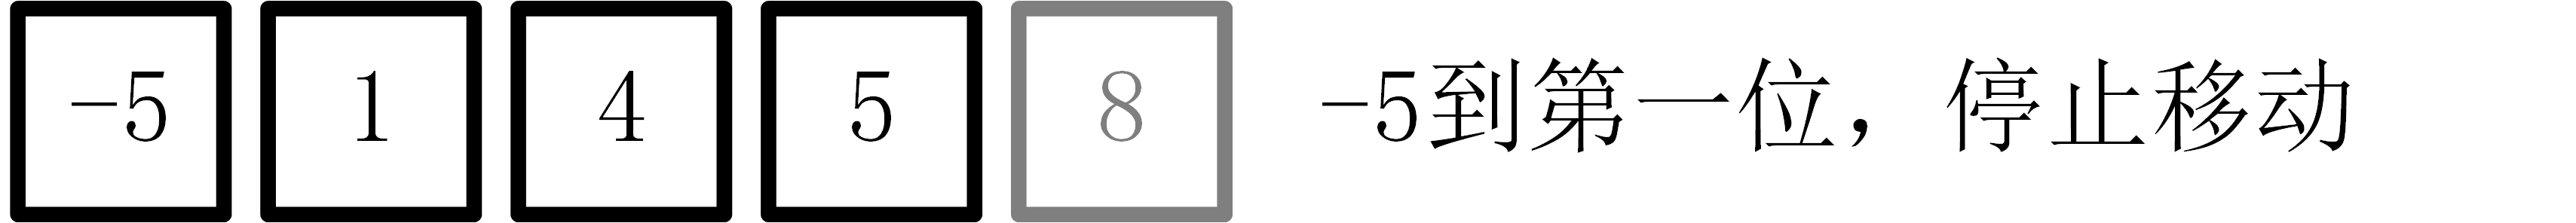
\includegraphics[width=0.8\textwidth]{insertion_sort_11}}\\\vspace{3mm}
%\uncover<12->{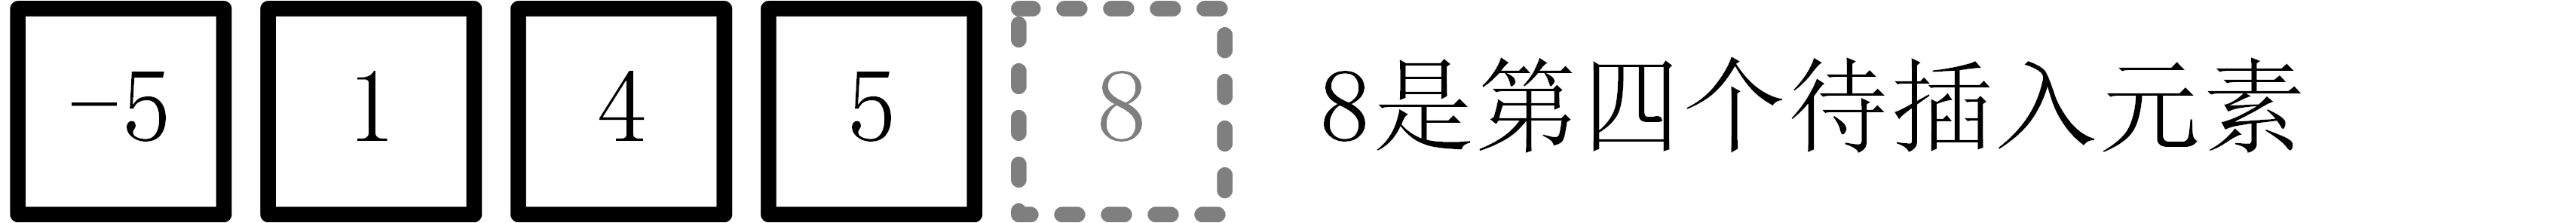
\includegraphics[width=0.8\textwidth]{insertion_sort_12}}\\\vspace{-10.9mm}
%\uncover<13->{
\includegraphics[width=0.8\textwidth]{insertion_sort_13}}
%\end{center}
%
%\end{frame}
%
%%-----------------
%
%\begin{frame}[fragile]{7.3.1 排序算法\normalsize{~---~插入排序}}
%
%插入排序算法的实现如下:
%
%\vspace{-4mm}
%
%\begin{columns}[t]
%
%\column{0.65\textwidth}
%\begin{blueblock}{\texttt{Array}成员函数\texttt{insertionSort}定义}
%\begin{lstlisting}[moreemph={Array,T,F}]
%template<typename T, size_t N>
%template<typename F >
%void Array<T, N>::insertionSort(F f) {
%    for (int i = 1, j; i < N; ++i) {
%        T t = m_ele[i]; //待插入元素
%        for (j = i; j > 0; --j) { //查找插入位置
%            if (f(m_ele[j - 1], t))
%                break;
%            m_ele[j] = m_ele[j - 1]; //逐个向后移动元素
%        }
%        m_ele[j] = t; //将待插入元素放到正确位置
%    }
%}
%\end{lstlisting}
%\end{blueblock}
%
%\column{0.3\textwidth}
%
%\end{columns}
%
%\end{frame}
%
%%-----------------
%
%\begin{frame}[fragile]{7.3.1 排序算法\normalsize{~---~冒泡排序}}
%
%不断比较相邻的两个元素,如果发现逆序则交换
%
%\vspace{1mm}
%
%\begin{center}
%
\includegraphics[width=0.8\textwidth]{bubble_sort_1}\\\vspace{3mm}
%\uncover<2->{
\includegraphics[width=0.8\textwidth]{bubble_sort_2}}\\\vspace{-10.9mm}
%\uncover<3->{
\includegraphics[width=0.8\textwidth]{bubble_sort_3}}\\
%\uncover<4->{
\includegraphics[width=0.8\textwidth]{bubble_sort_4}}\\\vspace{-10.9mm}
%\uncover<5->{
\includegraphics[width=0.8\textwidth]{bubble_sort_5}}\\
%\uncover<6->{
\includegraphics[width=0.8\textwidth]{bubble_sort_6}}\\\vspace{-10.9mm}
%\uncover<7->{
\includegraphics[width=0.8\textwidth]{bubble_sort_7}}\\
%\uncover<8->{
\includegraphics[width=0.8\textwidth]{bubble_sort_8}}\\\vspace{3mm}
%\uncover<9->{
\includegraphics[width=0.8\textwidth]{bubble_sort_9}}
%\end{center}
%
%\end{frame}
%
%%-----------------
%
%\begin{frame}[fragile]{7.3.1 排序算法\normalsize{~---~冒泡排序}}
%
%冒泡排序算法的实现如下:
%
%\vspace{-4mm}
%
%\begin{columns}[t]
%
%\column{0.65\textwidth}
%\begin{blueblock}{\texttt{Array}成员函数\texttt{selectionSort}定义}
%\begin{lstlisting}[moreemph={Array,T,F}]
%template<typename T, size_t N>
%template<typename F >
%void Array<T, N>::bubbleSort(F f){
%    for (int i = N - 1; i >= 0; --i){
%        for (int j = 0; j <= i - 1; ++j){
%            if (f(m_ele[j + 1], m_ele[j]))
%                swap(j, j + 1); //相邻元素交换
%        }
%    }
%}
%\end{lstlisting}
%\end{blueblock}
%
%\column{0.3\textwidth}
%
%\end{columns}
%
%\end{frame}
%
%%-----------------
%
%\begin{frame}[fragile]{7.3.1 排序算法\normalsize{~---~快速排序}}
%
%\begin{block}<1->{快速排序}
% 快速排序是冒泡排序的改进,在排序过程中数据移动少。\\
%\end{block}
%\begin{block}<2->{快速排序的基本思想}
%基本思想:划分和分治递归。\\
%   \begin{enumerate}
%     \item 划分:将整个数组划分为两个部分,第一部分所有值小于基准值(key),第二部分所以值大于基准值(key)。(基准值的选择是随机的,一般选择待排数组的第一个元素)。
%     \item 分治递归:第一步将数组划分为两部分后,两部分内部还不是有序的,再分别对两部分递归地进行快速排序,最终得到一个完整的有序数组
%   \end{enumerate}
%\end{block}
%\end{frame}
%
%\begin{frame}[fragile]{7.3.1 快速排序}
%
%\begin{block}{快速排序的流程}
%(1)left、right指针(索引)分别指向待排数组的首、尾。\\
%(2)left 指针向后遍历,right指针向前遍历。\\
%(3)当right指针指向元素小于基准值(key)时,right指针元素便赋值给left指针元素,完成转移。\\
%(4)当left指针指向元素大于基准值(key)时,left指针元素便赋值给right指针元素,完成转移。\\
%(5)最终当left=right时,遍历结束。\\
%(6)以基准值(key)为界限,把数组分成两部分,分别对这两部分进行快速排序(显然这是一个递归的过程)\\
%\end{block}
%
%\end{frame}
%\begin{frame}[fragile]{7.3.1 快速排序}
%\begin{center}
% 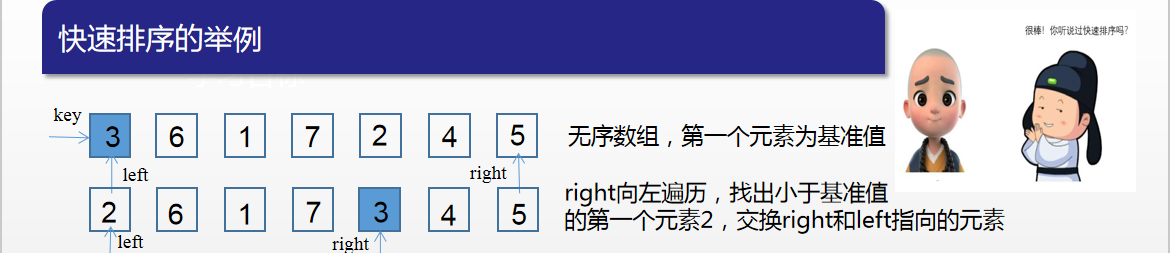
\includegraphics[scale=0.38]{quick_sort_1.png}\\
%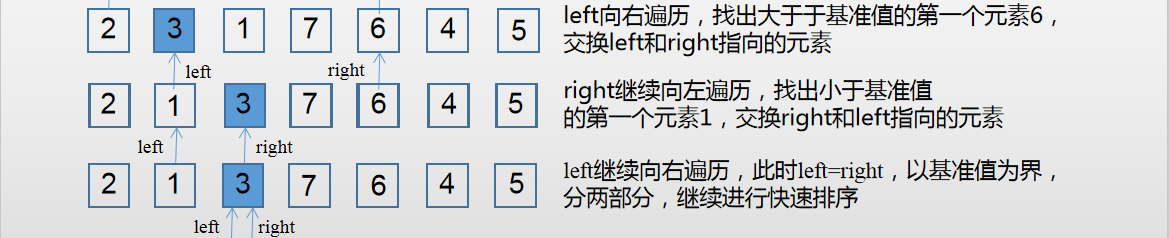
\includegraphics[scale=0.38]{quick_sort_2.png}
%\end{center}
%\end{frame}
%\begin{frame}[fragile]{7.3.1快速排序}
%\begin{block}{快速排序的举例续}
%\end{block}
%\begin{center}
%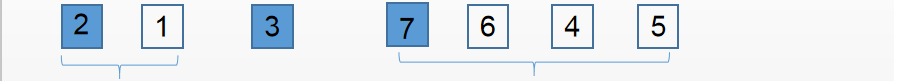
\includegraphics[scale=0.38]{quick_sort_6.png}
%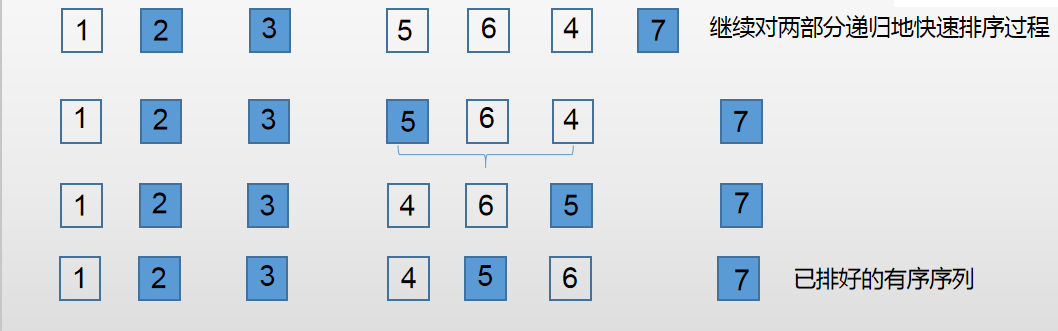
\includegraphics[scale=0.38]{quick_sort_7.png}
%\end{center}
%\end{frame}
%
%%\begin{frame}[fragile]{7.3.1 快速排序}
%%\begin{block}{快速排序的小技巧}
%%(1)若以数组的第一个元素为基准值,则应该先用right向左遍历,然后再用left向右遍历。\\
%%~\\
%%(2)若以数组的最后一个元素为基准值,则应该先用left向右遍历,然后再用right向左遍历。\\
%%~\\
%%(3)一般不建议用数组中间的元素做基准值,但也可以用。\\
%%~\\
%%\end{block}
%%
%%\end{frame}
%%\begin{frame}[fragile]{7.3.1 快速排序}
%%~\\
%%~\\
%%\begin{center}
%%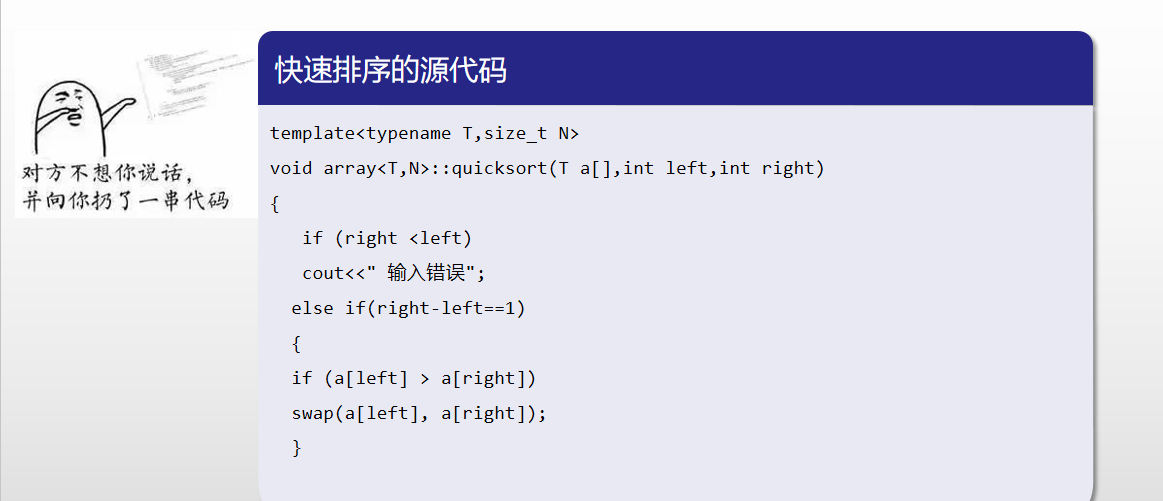
\includegraphics[scale=0.3]{quick_sort_3.png}
%%\end{center}
%%\end{frame}
%%\begin{frame}[fragile]{7.3.1快速排序}
%%~\\
%%~\\
%%\begin{center}
%%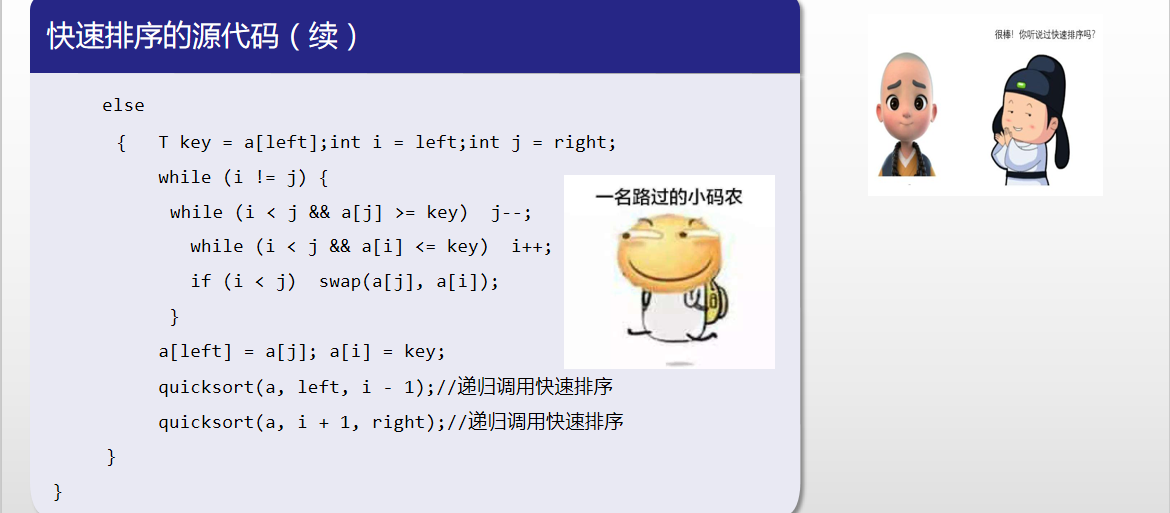
\includegraphics[scale=0.3]{quick_sort_4.png}
%%\end{center}
%%\end{frame}
%
%\begin{frame}[fragile]{7.3.1 快速排序}
%~\\
%~\\
%\begin{center}
%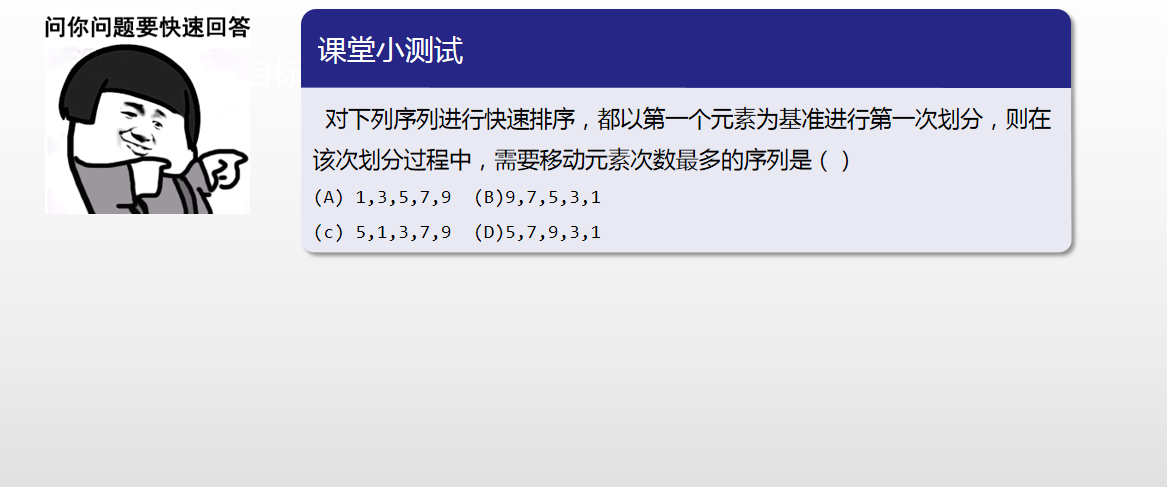
\includegraphics[scale=0.3]{quick_sort_5.png}
%\end{center}
%\end{frame}
%
%%-------------------------------------
%\subsection{二分查找算法}
%%-------------------------------------
%
%%-----------------
%
%\begin{frame}[fragile]{7.3.2~二分查找算法}
%
%又称折半查找,在有序序列中使用,其基本思想为分而治之
%
%\vspace{1mm}
%
%\begin{center}
%\uncover<2->{
\includegraphics[width=0.8\textwidth]{binary_search_1}}\\\vspace{3mm}
%\uncover<3->{
\includegraphics[width=0.8\textwidth]{binary_search_2}}\\\vspace{-10.2mm}
%\uncover<4->{
\includegraphics[width=0.8\textwidth]{binary_search_3}}\\\vspace{-10.2mm}
%\uncover<5->{
\includegraphics[width=0.8\textwidth]{binary_search_4}}\\\vspace{-10.2mm}
%\uncover<6->{
\includegraphics[width=0.8\textwidth]{binary_search_5}}\\\vspace{-10.mm}
%\uncover<7->{
\includegraphics[width=0.8\textwidth]{binary_search_6}}\\\vspace{12mm}
%\uncover<8->{
\includegraphics[width=0.8\textwidth]{binary_search_7}}\\\vspace{3mm}
%\uncover<9->{
\includegraphics[width=0.8\textwidth]{binary_search_8}}\\\vspace{-10.mm}
%\uncover<10->{
\includegraphics[width=0.8\textwidth]{binary_search_9}}\\\vspace{-10.mm}
%\uncover<11->{
\includegraphics[width=0.8\textwidth]{binary_search_10}}\\\vspace{-10mm}
%\uncover<12->{\includegraphics[width=0.8\textwidth]{binary_search_11}}\\\vspace{-10.mm}
%\uncover<13->{\includegraphics[width=0.8\textwidth]{binary_search_12}}\\\vspace{-10.mm}
%\uncover<14->{\includegraphics[width=0.8\textwidth]{binary_search_13}}\\\vspace{-10.mm}
%\uncover<15->{\includegraphics[width=0.8\textwidth]{binary_search_14}}\\\vspace{-10.mm}
%\end{center}
%
%\end{frame}
%
%%-----------------
%
%\begin{frame}[fragile]{7.3.2~二分查找算法}
%
%二分查找算法的实现如下:
%
%\vspace{-4mm}
%
%\begin{columns}[t]
%
%\column{0.65\textwidth}
%\begin{blueblock}{\texttt{Array}成员函数\texttt{binarySearch}定义}
%\begin{lstlisting}[moreemph={Array,T,F}]
%template<typename T, size_t N>
%int Array<T, N>::binarySearch(const T &value, int left, int right) {
%    while (left <= right) {
%        int middle = (left + right) / 2;//计算中点位置
%        if (m_ele[middle] == value)
%            return middle;
%        else if (m_ele[middle] > value)
%            right = middle - 1;//修改right
%        else
%            left = middle + 1;//修改left
%    }
%    return -1; //查找失败
%}
%\end{lstlisting}
%\end{blueblock}
%
%
%\column{0.3\textwidth}
%\begin{yellowblock}{说明}
%$\bullet$ 如果\texttt{value}小于中点位置(\texttt{middle})元素,则将\texttt{right}设为\texttt{middle-1}\\
%$\bullet$ 如果\texttt{value}大于中点位置元素,则将\texttt{left}设为\texttt{middle+1}\\
%$\bullet$ 如果查找失败则返回\texttt{-1}
%\end{yellowblock}
%\vspace{-2mm}
%\begin{greenblock}<2->{问题}
%查找\texttt{4}返回时,\texttt{left}和\texttt{right}的值是多少?
%\end{greenblock}
%\vspace{-2mm}
%\begin{greenblock}<3->{答案}
%\texttt{left}为\texttt{2},\texttt{right}为\texttt{1}
%\end{greenblock}
%
%\end{columns}
%
%\end{frame}
%
%-----------------

\begin{frame}[c]{~}
\begin{center}
  \huge{本章结束}
  \begin{block}{作业}
 \begin{enumerate}
   \item 在线提交系统:第七章作业
   \item 检查日期:待定
 \end{enumerate}
\end{block}
\end{center}
\end{frame}

%----------------------------------------------------------------------------------------

\end{document}
